% Template author: Johannes Demel
% Document class provides standardized title page + needed extras.
\documentclass{cel-thesis/cel-thesis}
\thesisTitle{Write my thesis}
\thesisType{Example Template}
\thesisAuthor{Moritz Luca Schmid}
%\thesisAdvisor{Univ.-Prof. i. R. Dr.rer.nat. Friedrich K. Jondral}
%\thesisHeadOfInstitute{Dr.-Ing. Holger Jäkel}
\thesisSupervisor{M.Sc. Felix Wunsch}
\thesisStartDate{12.06.2017}
\thesisEndDate{12.12.2017}
\thesisSignatureDate{31.11.2015}
\thesisLanguage{ngerman} % english or ngerman
\thesisCC{FALSE}
\thesisPythonWatermark{FALSE}


%%% LANGUAGE SETTINGS %%%%%%%%%%%%%%%%%%%%%%%%%%%%%%%%%%%%%%%%%%%%%%%%%%%%%
% additional Hyphenation rules
\hyphenation{non-para-metric repro-gra-mmable}
% Settings for bibliography
\usepackage{babelbib}
\setlanguage % set correct language as selected above

%%% PACKAGES %%%%%%%%%%%%%%%%%%%%%%%%%%%%%%%%%%%%%%%%%%%%%%%%%%%%%%%%%%%%%%%%%
% Add all the packages you feel like you need them.
% You'll need it.
% automatically expand/abbreviate terms.
\usepackage{caption}
\usepackage{subcaption}
\usepackage{todonotes} % great for draft annotations
%\usepackage[latin1]{inputenc}
\usepackage{tikz}
\usepackage{mathtools}
\usepackage{amsmath}
\usepackage{amsfonts}
\usepackage{siunitx}
\usepackage{pgfplots}
\usepackage{filecontents}
\usepackage{tikz}
\usetikzlibrary{datavisualization}


%%% DEFINITIONS %%%%%%%%%%%%%%%%%%%%%%%%%%%%%%%%%%%%%%%%%%%%%%%%%%%%%%%%%%%%%%%%%
%% pretty C++ print.
\def\CC{{C\nolinebreak[4]\hspace{-.05em}\raisebox{.4ex}{\tiny\textbf{++}}}}

\begin{document}
\pagenumbering{roman}  % all the preliminaries should be counted roman style
\maketitle
%% preliminaries
  \chapter*{Abstract}
This is my abstract.
CEL thesis rules require it to be about 3-5 pages. \todo{This is a todo example}
It is a summary of what you do in your thesis.
Use around 5 pictures and outline whatever you did.
And now a few lines of information.


		% a MUST, few pages abstract

%% main document
\cleardoublepage
\pagenumbering{arabic} % now old school arabic enumerated pages.
  \tableofcontents 		% a MUST
  \cleardoublepage		% make sure multipage TOCs are numbered correctly.
  \chapter{Einführung}
\label{sec:intro}
\ac{DAB} ist ein Übertragungsstandard zur Verbreitung von digitalem Radio. Das System wurde in den 90er Jahren im Zuge des Eureka 147 DAB Projekts entwickelt und kommt seit 1997 in vielen Teilen Europas und Asiens zum Einsatz. Mit dem DAB+ System, das eine Weiterentwicklung von DAB darstellt, soll langfristig die analoge \acp{UKW} Übertragung ersetzt werden.\\
Die digitale Datenübertragung bietet dabei eine verbesserte Audioqualität, da Übertragungsfehler durch Codierung empfängerseitig korrigiert werden können und somit nicht zu einem verrauschten Audiosignal wie bei FM führen. Eine Audiokompression verringert zusätzlich die Datenrate, was sich in einer gesteigerten spektralen Effizienz pro Audiokanal widerspiegelt. Die digitale Übertragung bietet außerdem viele neue Möglichkeiten der medialen Unterstützung in Form von Service Informationen wie Albumcovers, ausführlichen Stauinformationen oder Wetterkarten.\\
DAB Sender sind in sog. Ensembles strukturiert. Ein DAB Ensemble enthält ein ganzes Multiplex an Audio- und Datenkanälen. Radiosender dieses Ensembles greifen auf eine Auswahl dieser Kanäle zu. Dieses dynamische Multiplex erlaubt eine flexible und individuelle Programmgestaltung. \\
DAB stellt vier verschiedene Übertragungsmodi zur Verfügung, die für verschiedene Ausbreitungsszenarien und Frequenzbereiche ausgelegt sind. Der Fokus liegt dabei auf dem mobilen Empfang bei terrestrischer Übertragung, es existiert aber auch jeweils ein Modus für die Satellitenübertragung, sowie die niederfrequente Übetragung per Kabel. Eine Besonderheit bei DAB stellt der Einsatz von sog. Single Frequency Networks (SFNs) dar, bei denen eine Vielzahl von örtlich getrennten Sendestationen auf der gleichen Frequenz ausstrahlen. Dadurch kann ein enormer Gewinn an Frequenzeffizienz erzielt werden. Der Einsatz von SFNs wird bei DAB durch eine hohe Robustheit des Übertragungssystems gegenüber Mehrwegeempfang ermöglicht \cite{dab_buch}.\\
Ziel dieser Arbeit ist die Implementierung und Evaluation eines Senders und Empfängers für DAB/DAB+. Die Implementierung wird dabei in Form eines Software Defined Radios erfolgen, einem System bei dem ein Großteil der Signalverarbeitung auf Softwareebene durchgeführt wird. Dazu wird die Open-Source Software GNU Radio verwendet. Im Weiteren soll eine grafische Transceiver Applikation realisiert werden, die auf Basis des implementierten Senders und Empfängers eine benutzerfreundliche Oberfläche für das Senden und das Empfangen von DAB/DAB+ Signalen darstellt.

		% include chapter introduction.tex
  \let\conjugatet\overline
\chapter{Implementierung}
\todo{Signalmodell, Annahmen, Einflüsse, usw}
\begin{figure}[ht]
\centering
  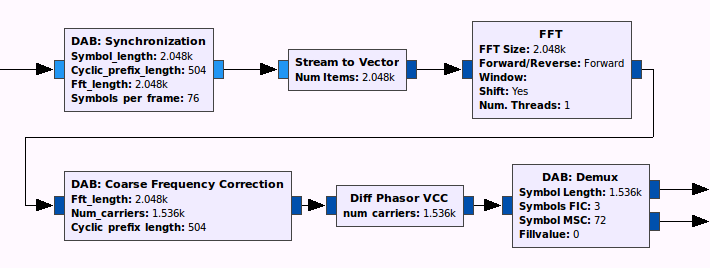
\includegraphics[width=0.8\textwidth]{figures/sync_hier_block.png}
	\caption{Aufbau der kompletten Synchronisationskette im \ac{GRC}}
	\label{fig:sync_overview}
\end{figure}

\section{OFDM}
\subsection{Zeit Synchronisation}
Eine geeignete Zeitsynchonisation muss sowohl eine grobe Synchronisation des OFDM Frames als auch eine feine Synchonisation der einzelnen OFDM Symbole sicherstellen. \\

Der Beginn eines jeden Frames $ k $ wird durch das Nullsymbol $z_{0,k}$ markiert. Wegen $S(t) = 0$ für $t \in [0, T_{NULL}]$ stellt es eine zuverlässige Möglichkeit dar den Anfang eines Frames über eine Energiemessung zu detektieren.
\todo{Formel Energie aber Intervall kürzer als T NULL}

\begin{equation}
E[i] = \sum \limits_{j=i}^{T_G}|x[j]|^2
\label{eq:energy}
\end{equation}

Nachdem der Anfang eines Frames detektiert wurde, muss im Folgenden der Beginn jedes OFDM Symbols $z_{l,k}$ ($l \in [1, 76]$) festgelegt werden. Diese feine Zeitsynchronisation erfordert keine sehr hohe Genauigkeit, da jedem Symbol ein Cyclic Prefix der Dauer $T_G = 246 \mu s $ vorgeschoben ist, dessen Inhalt dem Ende des eigentlichen Symbols entspricht. Dadurch ergibt sich ein Zeitbereich von  $T_D \in [0,T_G]$ in dem das Symbol fehlerfrei gesetzt werden kann, also das gesetzte Symbolfenster nicht in das vorhergehende oder nachfolgende Symbol hereinragt.

% cyclic prefix figure
\begin{figure}
\begin{center}
\begin{tikzpicture}
\newcommand{\ursprung}{(0,0)}
\node[] at \ursprung (null) {}; 
\draw [thick, rounded corners = 6pt] 
    (null) -- ++(0,0.5) -- ++(0,0.5) -- ++(8,0) -- ++(0,-1) -- ++(-8,0) -- ++(0,0.5);
\draw [dashed]
    (null)+(2,0) -- ++(2,1);
\draw [dashed]
    (null)+(6,0) -- ++(6,1);
\node[] at (1,1.5) (guard) {$T_G$};
\draw [<-] (0,1.5) -- (guard.west);
\draw [->] (guard.east) -- (2,1.5);
\node[] at (5,1.5) (symbol) {$T_S$};
\draw [<-] (symbol)+(-3,0) -- (symbol.west);
\draw [->] (symbol) -- (8,1.5);
\node[] at (0.75,-0.5) (delay) {$T_D$};
\draw [<-] (delay)+(-0.75,0) -- (delay.west);
\draw [->] (delay) -- (1.5,-0.5);
%Beschriftung
\node[] at (1,0.5) (cp) {CP};
\node[] at (7,0.5) (cp) {CP Quelle};
%Vorgängersymbol
\draw [thick, rounded corners = 6pt]
    (-1.5,0) -- ++(1.5,0) -- ++(0,1) -- ++(-1, 0);
\draw [decorate,decoration={snake, amplitude=.4mm}] (-1.5,0) -- (-1,1);
%Nachfolgersymbol
\draw [thick, rounded corners = 6pt]
    (9,0) -- ++(-1,0) -- ++(0,1) -- ++(1.5, 0);
\draw [decorate,decoration={snake, amplitude=.4mm}] (9,0) -- ++(0.5,1);
%gesetztes Symbolfenster
\draw[-,decorate,decoration=brace] 
    (7.5,-0.2) -- (1.5,-0.2) node [midway, yshift=-0.3cm]{};
\node[] at (4.5,-0.6) {gesetztes Symbolfenster für $z_{l,k}$};
\end{tikzpicture}
\end{center}
\caption{OFDM Symbol und Cyclic Prefix}
\label{chart:cp}
\end{figure}

Um \ac{ISI} zu minimieren ist der theoretisch optimale Abtastzeitpunkt genau am Ende des Cyclic Prefix zu wählen. Eine komplette \ac{ISI} Unterdrückung ist wegen $T_G < \tau_{max}$ mit einer maximalen Echo Verzögerung von $\tau_{max} = 300 \mu s$ \todo{cite} nicht möglich. Jedoch wird die \ac{ISI} zu einem Minimum reduziert, wenn ein maximal später Startpunkt gewählt wird, da dadurch die Interferenzzeit $\tau_{max} - T_G$ (bei $\tau_{max} < T_G+T_S$) minimiert wird.

\todo{Bild mit Symbol und evt Frame, wo Zeitreferenz markiert ist, auf dem dann die Formeln/Delays basieren können}

Um den exakten Anfang eines Symbols zu bestimmen, wird die zyklische Wiederholung des Symbolanteils im Cyclic Prefix genutzt. Durch eine Korrelation des abgetasteten Empfangssignal $x[i]$ mit einer um $T_S$ verzögerten Version desselben Signals $x[i+T_S]$ über das Intervall $[i, i+T_G]$ kann der Anfang des Cyclic Prefix über einen Peak der Korrelation identifiziert werden.

\todo{klären, wann $T_G$ Zeit und wann samples angibt, bzw anderes symbol verwenden}
%einfache correlation
\begin{equation}
y[i] = \sum \limits_{j=i}^{T_G}r[j] \conjugatet{r[j+T_S]}, \ \ y[i] \in \mathbb{C}
\label{eq:corr_einfach}
\end{equation}

Unter Berücksichtigung von additivem weißen Rauschen r[i]=x[i]+n[i] mit $N[i] \sim \mathcal{N}(\mu,\,\sigma^{2})$ ergibt sich

\begin{equation}
    \begin{aligned}
y[i] &= \sum \limits_{j=i}^{T_G}(x[j]+N[j]) \conjugatet{(x[j+T_S]+N[j])} \\
&= \sum \limits_{j=i}^{T_G}x[j] \conjugatet{x[j+T_S]} + \sum \limits_{j=i}^{T_G}x[j] \conjugatet{n[j+T_S]} + \sum \limits_{j=i}^{T_G}n[j] \conjugatet{x[j+T_S]} + \sum \limits_{j=i}^{T_G}n[j] \conjugatet{n[j+T_S]} \\
&= P T_G + 2(P \sigma^2) + \sigma^4 \approx P T_G + 2(P \sigma^2)
    \end{aligned}
\end{equation}

und damit ein SNR des Korrelationssignals von
\begin{equation}
SNR = \frac{P_x}{P_n} = \frac{P T_G}{2 P \sigma^2} = \frac{T_G}{2 \sigma^2}
\end{equation}

Durch eine Mittelung über $T_G * Samplerate = 504$ Samples ist das SNR somit ausreichend groß um eine entprechend genaue Peakdetektion durchführen zu können.

\begin{figure}[ht]
\centering
  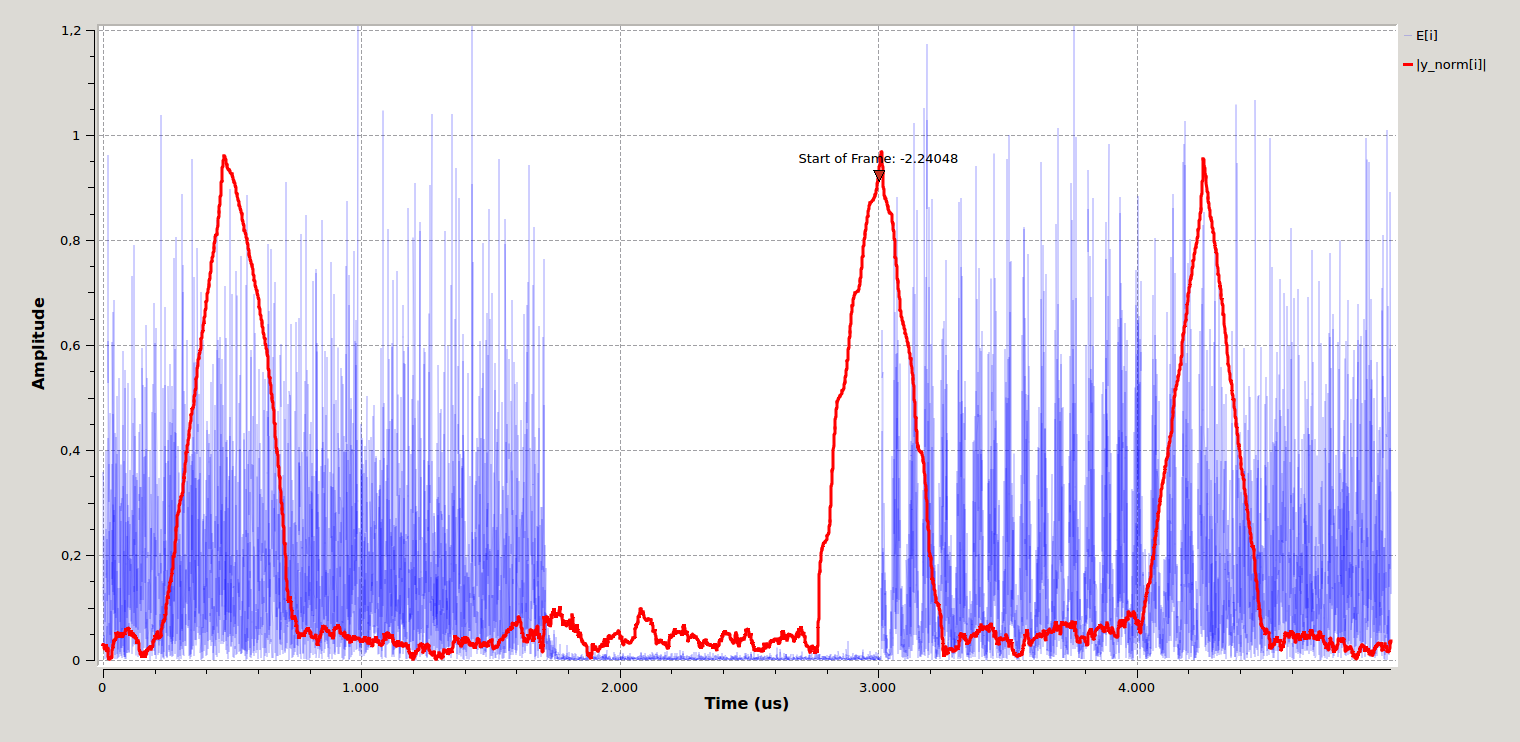
\includegraphics[width=0.8\textwidth]{figures/delayed_correlation_abs_and_energy.png}
	\caption{Korrelation des Cyclic Prefix}
	\label{fig:corr}
\end{figure}

Die Korrelation ist dabei auf die Energieanteile des Cyclic Prefixes und dessen Quelle nach $T_S$ normiert, sodass das Ergebnis unabhängig von der Empfangsleisung bleibt, die durch Empfangsqualität und verwendeter Hardware stark variieren kann.

\begin{equation}
    y_{norm}[i] = \frac{\sum \limits_{j=i}^{T_G}x[j] \conjugatet{x[j+T_S]}}{\sqrt{\sum \limits_{j=i}^{T_G}|x[j]|^2 \sum \limits_{j=i}^{T_G}|x[j+T_S]|^2}} = \frac{\sum \limits_{j=i}^{T_G}x[j]     \conjugatet{x[j+T_S]}}{\sqrt{E[i]E[i+T_S]}}
    \label{eq:norm_corr}
\end{equation}

In Abbildung~\ref{fig:corr} ist zu erkennen, dass die Flanken der Korrelation linear ansteigen. Die Breite einer Flanke entspricht $T_G$, also gerade dem Entscheidungsbereich für $T_D$. Durch die Linearität der Flanke und der Normierung, kann der relative Abtastzeitpunkt innerhalb des Cyclic Prefix über einen Schwellwert eingestellt werden. Der tatsächliche Abtastzeitpunkt wird anschließend mit einer Verzögerung von $T_G$ gestetzt. In der Implementierung von Abbildung~\ref{fig:corr} wurde ein Schwellwert von $0,85$ eingestellt, der sich als guter Kompromiss zwischen \ac{ISI} Unterdrückung und einem Sicherheitsabstand zu $T_D > T_G$ herausgestellt hat. Man beachte, dass $T_D > T_G$ dazu führt, dass Samples vom nachfolgenden Symbol im gesetzen Symbolfenster liegen was zum Empfang von falscher Information führt. Dieser Fall entspricht einer fehlerhaften Zeitsynchronisation.

\subsubsection{Implementierung}
Um eine mehrfache Berechnung von Gleichung~\ref{eq:energy} für die Energiemessung (Gl.~\ref{eq:energy}) sowie die normierte Korrelation (Gl.~\ref{eq:norm_corr}) zu vermeiden, wurde die feine und grobe Zeitsynchronisation in einer gemeinsamen Klasse implementiert.

\begin{figure}
\begin{center}
\begin{tikzpicture}[node distance = 2cm, auto]
% Define block styles
\tikzstyle{decision} = [diamond, draw, fill=cyan!30, 
    text width=4.5em, text badly centered, node distance=3cm, inner sep=0pt]
\tikzstyle{start} = [rectangle, draw, fill=cyan!30, 
    text width=5em, text centered, rounded corners, minimum height=4em]
\tikzstyle{output} = [trapezium, draw, fill=cyan!30, 
    text width=4em, text centered, minimum height=4em, trapezium right angle=110, trapezium left angle=70]
\tikzstyle{block} = [rectangle, draw, fill=cyan!30, 
    text width=5em, text centered, minimum height=4em]
\tikzstyle{line} = [draw, -latex']
\tikzstyle{cloud} = [draw, ellipse,fill=red!20, node distance=3cm,
    minimum height=2em]
    % Place nodes
    \node [start] (init) {Start};
    \node [decision, below of=init] (null) {NULL erwartet?};
    \node [block, below of=null, node distance=3cm] (corr) {gleitende Korrelation};
    \node [decision, below of=corr, node distance=3cm] (peak) {Peak?};
    \node [block, below of=peak, node distance=2.5cm] (energy) {Energie- messung};
    \node [decision, below of=energy] (first) {Symbol $z_{1,k}$?};
    \node [output, below of=first, node distance=3cm] (tag) {Start des Frames in $T_G$};
    \node [block, right of=null, node distance=4.5cm] (skip) {überspringe $T_S$};
    \node [block, below of=skip, node distance=3cm] (corr2) {einmalige Korrelation};
    \node [decision, below of=corr2] (peak?2) {Peak?};
    \node [above of=null, node distance=2cm] (backtonull){};
    \node [output, below of=peak?2, node distance=3cm] (lost track){nicht mehr in Sync};
    
    \path [line] (init) -- (null);
    \path [line] (null) -- node {ja} (corr);
    \path [line] (null) -- node {nein} (skip);
    \path [line] (corr) -- (peak);
    \path [line] (peak) -- node {ja} (energy);
    \path [line] (energy) -- (first);
    \path [line] (first) -- node {ja} (tag);
    \path [line] (peak) -- node {nein} ++(2.5cm,0);
    \path [line] (first) -- node {nein} ++(2.5cm,0) |- (corr);
    \path [line] (skip) -- (corr2);
    \path [line] (corr2) -- (peak?2);
    \path [line] (peak?2.south) -- node {nein} (lost track);
    \path [line] (peak?2.east) -- node{ja}++(1cm,0) -- ++(0,8cm) -- ++(-6.5,0);
    \path [line] (tag) -- node{}++(0,-1cm) -- node {} ++(-2.5cm,0) -- node{}++(0,17.5cm) -- ++(2.5cm,0);
    \path [line] (lost track.south) -- ++(0,-1cm) -- ++(-2,0);
\end{tikzpicture}
\end{center}
\caption{Programmablaufplan der Zeitsynchronisation}
\label{chart:zeitsync}
\end{figure}

Abbildung~\ref{chart:zeitsync} zeigt den Programmablaufplan der Zeitsynchronisation. Er ist aufgeteilt in die beiden Zweige "Suche Frame Start" und "Kontrolle". Der Zweig "Suche Frame Start" kommt bei einem der folgenden Fälle zum Einsatz:
\begin{itemize}
\item Die Synchronisation wird initial gestartet.
\item Das Programm ist nicht mehr in Synchronisation.
\item Das Ende eines Frames wurde erreicht.
\end{itemize}
Alle diese Situationen haben gemeinsam, dass im Folgenden nach dem Peak des Symbols $z_1,k$ (erstes Symobl nach dem Nullsymbol) gesucht wird. Es wird iterativ für jedes Sample des Zeitsignals $x[i]$ eine Korrelation $y[i]$ nach Gl.~\ref{eq:norm_corr} durchgeführt. Dadurch können (analog zu Abb.~\ref{fig:corr}) Korrelationspeaks detektiert werden die jeweils dem Start eines Symbols entsprechen. Durch die Energiemessung das Symbols $z_{1,k}$ von den restlichen Symbolen $z_{l,k},$ mit  $l \in [2,76]$ unterschieden werden.

Die Komplexität der Korrelationsoperation kann drastisch reduziert werden, indem die Summe, die laut Gl.~\ref{eq:corr_einfach} in jedem Schritt $T_G = 504$ Additionen durchführt, durch eine gleitende Summe ersetzt wird.
%gleitende Summe
\begin{equation}
    y[i+1] = y[i] - r[i] \conjugatet{r[i+T_S]} + r[i+T_G] \conjugatet{r[i+T_G+T_S]}
    \label{eq:moving_sum}
\end{equation}
Dabei ist zu beachten, dass natürlich $y[i=0]$ komplett berechnet werden muss. Um einen das Ergebnis verfälschenden Drift von $y[i]$ zu vermeiden, wird die Summe außerdem alle $i=100000$ Samples neu berechnet.

Wenn der Anfang von $z_{1,k}$ gefunden und festgelegt wurde, stehen auch die Anfänge aller anderen Symbole des Frames fest, da sie mit dem festen und bekannten Abstand von $T_G+T_S$ direkt aufeinanderfolgen. Der Zweig "Kontrolle" springt daher nur noch vom Start eines Symbols $x[i]$ zum Nächsten $x[i+T_G+T_S]$ und berechnet an dieser Stelle einmalig die Korrelation $y[i+T_G+T_S]$. Liegt $y[i+T_G+T_S]$ über einem Schwellwert, wurde das Sample als Anfang des nächsten Symbols bestätigt und die Kontrollschleife iteriert zum nächsten Symbol. Falls an einem erwarteten Symbolanfang der Schwellwert der Korrelation unterschritten wird, wechselt das Programm in den Zweig "Suche Frame Start".

Da die Symboldauer genau bekannt ist, mag eine Kontrolle von jedem einzelnen Symbol zunächst überflüssig erscheinen. Der Aufwand wird jedoch gerechtfertigt um Störeffekte wie einen Clockdrift rechtzeitig erkennen und korrigieren zu können bevor dieser zu einem Verlust der Synchronisation und damit zu Datenverlusten führen kann.
Ein beispielhafter Clockdrift von 50 ppm kann im rauschfreien Fall zu einem maximalen Phasenfehler von
\begin{equation}
\begin{aligned}
    \Delta\varphi_{max} = 2 \pi f_{max} \Delta t &= 2 \pi \frac{B}{2} Clockdrift (T_G+T_S) \\
    &=  2 \pi \frac{1536 Hz}{2} 50ppm 1246\mu s \\
    &= 0,3 rad = \ang{17,2}
    \end{aligned}
    \label{eq:clockdrift}
\end{equation}
führen. Rechnung~\ref{eq:clockdrift} zeigt, dass eine feine Zeitsynchronisation zu jedem Framebeginn zu wenig ist, da sich der Phasenfehler bei 76 Symbolen pro Frame aufsummiert und damit die Entscheidungsgrenzen einer QPSK Demodulation überschreitet. Damit ist der Zweig "Kontrolle" gerechtfertigt.


%%%%%%%%%%%%%%%%%%%%%%%%%%%%%%%%%%%%%%%%%%%%%%%%%%%%%%%%%%%%%%%%%%%%%%%%%%%%%%%%%%%%%%%%%%%%%%%%%%%
\subsection{Frequenz Synchronisation}
Die Messung und Korrektur eines Frequenzoffsets ist der nächste Schritt der Synchronisationskette. Sie spielt in OFDM Systemen eine besonders wichtige Rolle, da ein Frequenzoffset die Orthogonalität zwischen den Unterträgern zerstört und somit zu \ac{ICI} führt.

\subsubsection{Feine Frequenz-Schätzung}
Für die Messung des Frequenzoffsets kann wieder auf die Korrelaton aus Gl.~\ref{eq:corr_einfach} zurückgegriffen werden. Ein Frequenzoffset lässt sich hier als konstante Änderung der Phase über der Zeit $T_S$ messen, da die Phase von Cyclic Prefix und dessen Wiederholung ohne Frequenzoffset gleich sind. 
\begin{equation}
f_{off}[i] = \frac{arg(y[i])}{T_S}
\label{eq:fine_frequency_estimation}
\end{equation}
Ein zusätzliches \ac{AWGN} ändert die Phase jedes einzelnen Samples. Wegen der Mittelwertfreiheit von \ac{AWGN} kann die Varianz des gemessenen Frequenzoffsets durch eine Mittelung reduziert werden.
\todo{Rechnung zu Varianz bei Mittelung (Gleichverteilung mit unabh. ZVs als Ausgangspunk}
Durch das Korrelationsintervall von $T_G = 504$ Samples wird solche eine Mittelung durchgeführt was die relativ kleine Varianz der Frequenzoffsetmessung in Abb.~\ref{plot:varianz_freq_offset} bestätigt.
\todo{Wie korrigieren reinbringen}
\begin{center}
\begin{tikzpicture}
\begin{axis}[
title=Varianz der feinen Frequenzoffsetmessung,
xlabel={$SNR \ [dB]$},
ylabel={$E((\hat{f} - f_{off})^2) \ [Hz]$},
grid=both,
]
\addplot [blue, mark=diamond*]table {data/171020_frequency_offset_variance.dat};
\end{axis}
\label{plot:varianz_freq_offset}
\end{tikzpicture}
\end{center}

Durch die aktive Mittelung über N Symbole wird eine weitere Senkung der Varianz um Faktor N erreicht. Pro Symbol wird genau eine Korrelation berechnet, also ergibt sich ein Mittelungsfenster der Dauer $N (T_G + T_S)$. Ein zu langes Mittelungsfenster führt zu einer Trägheit der Frequenzmessung und damit auch zu einer Zeitverzögerung in der Frequenzkorrektur, was bei schnellen Frequenzänderungen zu Synchronistaionsverlusten führen kann. Vor allem bei mobilen \ac{DAB} Empfängern wird dieser Fall aufgrund der Dopplerverschiebung relevant. Aus diesem Grund wird für die obere Grenze der Mittelung die Bedingung gestellt, dass bei einer maximalen, konstanten Beschleunigung $a$ der durch die Mittelung verursachte Messfehler $f_M$ unter der $3\sigma$ Grenze liegt.
\begin{equation}
f_M \overset{!}{<} \frac{3\sigma(SNR)}{\sqrt{N}}
\label{eq:3sigma_grenze}
\end{equation}
Mit $a=50m/s^2$ und einer Trägerfrequenz von $f_T = 200 MHz$ ist
\begin{equation}
\frac{df}{dt} = f_T * \frac{a}{c} = 33,3 Hz/s
\end{equation}
und damit
\begin{equation}
\begin{aligned}
f_M &= \frac{1}{N} \sum \limits_{i=0}^{N-1} i \frac{df}{dt} (T_G+T_S) \\
&= \frac{1}{N} \frac{df}{dt} (T_G+T_S) \left(\frac{N^2 + N}{2} - N\right) \ \ {\overset{N\text{groß}}{\approx}} \ \  \frac{df}{dt} (T_G+T_S) N
\end{aligned}
\label{eq:mittelung_fehler}
\end{equation}
Aus \ref{eq:3sigma_grenze} und \ref{eq:mittelung_fehler} ergibt sich eine rauschabhängige Obergrenze für das Mittelungsintervall.
\begin{equation}
N \overset{!}{<} \left(\frac{df}{dt}\frac{T_G + T_S}{3 \sigma(SNR)}\right)^{-2/3}
\end{equation}
 %%%%%%%%%%%%%%%%%%%%%%%%%%%%%%%%%%%%%%%%%%%%%%%%%%%%%%%%%%%%%%%%%%%%%%%%%%%%%%%%%%%%%%%%%%%
\subsubsection{Grobe Frequenz-Schätzung}
Wegen $arg(y[i]) \in (-\pi,\pi] rad$ ist der gemessene Frequenzoffset aus Gl.~\ref{eq:fine_frequency_estimation} nur in $f_{off} \in (-500,500] Hz$ eindeutig. Dieser Eindeutigkeitsbereich entpricht genau der Breite eines OFDM Unterträgers von $1 kHz$. Nach der feinen Frequenzkorrektur liegen also die Unterträger wieder auf dem Frequenzraster und es tritt durch die Orthogonalität keine ICI auf. Jedoch kann das Signal um das ganze Vielfache des Unterträgerabstandes verschoben sein, wodurch Symbole im Empfänger durch eine falsche Zuweisung der FFT Bins fehlinterpretiert würden und die komplette Information des Frames verloren ginge.
\todo{arctan bei Eindeutigkeit reinbringen?}
\todo{grobe fe nach FFT reinbringen}
Da sowohl die Erkenung als auch die Korrektur einer Unterträgerverschiebung im Frequenzbereich wesentlich einfacher und anschaulicher ist, wird die grobe Frequenz-Korrektur nach der FFT Operation (Abschn.~\ref{sec:FFT}) durchgeführt.
\todo{FFT Kapitel vorziehen?}
Von den 2048 Unterträgern die aus der FFT resultieren, sind jeweils die ersten $K = \frac{1536}{2}$ rechts und links des zentralen DC-Trägers belegt. Die restlichen, unbelegten Träger enthalten am Empfänger neben möglichst geringer \ac{ICI} lediglich \ac{AWGN}. Durch eine Korrelation des FFT Vektors mit dem Vektor der bekannten Trägerbelegung $[1,1,...,1,0,1,...,1,1]$ der Länge $1536+1$ kann der Trägeroffset n ermittelt werden.
\todo{evt Grafik mit beschriftung auf der die Beschreibung aufbauen kann, $T_u$ als FFT length definieren}
\begin{equation}
X[n] = \argmax_i \sum \limits_{n=i}^{i+K} |X[n]|^2 \ \ \text{mit} \ \ i \in [0,L_{FFT}-K)
\end{equation}

\subsection{FFT}
\label{sec:FFT}
Die modulierten Symbole werden durch das OFDM System parallel auf den $K=1536$ Unterträgern moduliert und sind innerhalb eines Sendesymbols $T_S$ durch ihre Phase und Frequenz vollständig beschrieben \cite{nt1}. Um aus dem empfangenen Zeitsignal nach der Zeit- und Frequenzsynchronisation nun wieder die D-QPSK Symbole zu erhalten, wechselt man mittels einer \ac{DFT} wieder in den Frequenzbereich, was in Gl.~\ref{eq:ofdm_dft} gezeigt wurde. Wegen $L_{DFT} = \frac{2,048 M samples/s}{T_S} = 2048 = 2^{11}$ kann die \ac{DFT} durch eine \ac{FFT} der Länge 2048 effizient implementiert werden. Der \ac{FFT} Algorithmus ist ist in GNU Radio \cite{repo:gr-fft} bereits implementiert und kann verwendet werden.
\todo{zitiere FFT aus SUS Buch}

\todo{Unbedingt Unterschiedliche Symbole für Zeit und Samples einführen!!!}

\subsection{Frequenzspreizung}
\subsection{Demodulation}
\subsection{Kanalcodierung}
\subsection{Audio Codecs}




  \acresetall
% This is an example chapter from 'Polar Codes for Software Radio'. Do not use it but delete it! It serves as an example!
\chapter{System model}\label{chapter:systemmodel}
Polar codes are defined for a specific system model.
The objective of this chapter is to introduce the key concepts.
Notations are introduced and important terms are revisited in order to refer to them.

\section{Key channel coding concepts}
The system model used throughout this thesis follows the remarks in \cite{Richardson:2008:MCT} and \cite{polar:arikan09}.
It is intended to define the domain for which polar codes are developed.

The objective of channel coding is to transmit information from a source to a sink over a point-to-point connection with as few errors as possible.
A source wants to transmit binary data  $u \in \mathcal{U} = \{0, 1\}$ to a sink where $u$ represents one draw of a binary uniformly distributed random variable.
The source symbols are encoded, transmitted over a channel and decoded afterwards in order to pass an estimate $\hat{u}$ to a sink.

This thesis uses a common notation for vectors which is introduced here shortly.
A variable $x$ may assume any value in an alphabet $x \in \mathcal{X}$.
Multiple variables are combined into a vector $x^N = (x_0, \dots , x_{N-1})$ of size $N$ with its alphabet $x^N \in \mathcal{X}^N$.
A subvector of $x^N$ is denoted $x_i^j = (x_i, \dots, x_{j-1})$ where $0 \leq i \leq j \leq N$.
A vector where $i=j$ is an empty vector.
A vector $x^N$ may be split into even and odd subvectors which are denoted $x_{0,e}^{2n} = (x_0, x_2, \dots, x_{2n-2})$, $x_{0,o}^{2n} = (x_1, x_3, \dots, x_{2n-1})$.
This numbering convention is in accordance with \cite{dijkstra:zerocounting}, where the author makes a strong point for this exact notation and some papers on polar codes follow it too, e.g. \cite{polar:talvardy:howtoCC}.


\subsection{Encoder}
The encoder takes a frame $u^k$ and maps it to a binary codeword $x^N$, where $k$ and $N$ denote the vector sizes of a frame and a codeword respectively with $k \leq N$.
An ensemble of all valid codewords for an encoder is a code $\mathcal{C}$.
It should be noted that $|\mathcal{C}| = |\mathcal{X}^N|$ must hold in order for the code to be able to represent every possible frame.

Not all possible symbols from $\mathcal{X}^N$ are used for transmission.
The difference between all possible codewords $2^N$ and used codewords $2^k$ is called redundancy.
With those two values, the code rate is defined as $R = \frac{k}{N}$.
It is a measure of efficient channel usage.

The encoder is assumed to be linear and to perform a one-to-one mapping of frames to codewords.
A code is linear if $\alpha x + \alpha' x' \in \mathcal{C}$ for $\forall x, x' \in \mathcal{C}$ and $\forall \alpha, \alpha' \in \mathbb{F}$ hold.
It should be noted that all operations are done over the Galois field GF(2) or $\mathbb{F} = \{0, 1\}$ if not stated otherwise.
Then the expression can be simplified to 
\begin{equation}
 x + x' \in \mathcal{C} \quad \textrm{for} \quad \forall x, x' \in \mathcal{C}.
\end{equation}
A linear combination of two codewords must yield a codeword again.

For linear codes it is possible to find a generator matrix $G \in \mathbb{F}^{k \times N}$ and obtain a codeword from a frame with $x^N = u^k G^{k \times N}$.
All linear codes can be transformed into systematic form $G = I_k P$.
$I_k$ is a $k \times k$ dimensional identity matrix.
If $G$ is systematic, all elements of a frame $u^k$ are also elements of the codeword $x^N$.
Also, a parity check matrix $H = -P^T I_{N-k}$ with dimensions $(N-k) \times N$ can be calculated from $G$.
A parity check matrix satisfies $\forall x \in \mathcal{C}: H x^T = 0^T $.
Thus, a parity check matrix can be used to verify correct codeword reception and furthermore error correction may be performed.
Error correction with $H$ may be done, e.g. syndrome decoding.

A code can be characterized by the minimum distance between any two codewords.
In order to obtain this value we use the Hamming distance.
This distance $d(v^N,x^N)$ equals the number of positions in $v^N$ that differ from $x^N$.
Minimum distance of a code is than defined by $d(\mathcal{C}) = \min\{d(x,v): x,v \in \mathcal{C}, x \neq v\}$.
For linear codes this can be simplified to comparing all codewords to the zero codeword $d(\mathcal{C}) = \min\{d(x,0): x \in \mathcal{C}, x \neq 0\}$ which is called Hamming weight.

\subsection{Channel model}\label{sec:channel_model}
Channel coding relies on a generic channel model.
Its input is $x \in \mathcal{X}$ and its distorted output is $y \in \mathcal{Y}$.
A channel is denoted $W: \mathcal{X} \rightarrow \mathcal{Y}$ along with its transition probability $W(y|x), x \in \mathcal{X}, y \in \mathcal{Y}$.
A \ac{DMC} does not have memory, thus every symbol transmission is independent from any other.
Combined with a binary input alphabet it is called a \ac{BDMC}.
For a symmetric channel model, $P(y|1) = P(-y|-1)$ must hold for an output alphabet $y \in \mathcal{Y}, \mathcal{Y} \subset \mathbb{R}$ \cite{Richardson:2008:MCT}.
Assuming symmetry for a \ac{BDMC} leads to a symmetric \ac{BDMC}.
In Sec. \ref{theory:channels} several examples of such channels are discussed.

This channel concept may be extended to vector channels.
A vector channel $W^N$ corresponds to $N$ independent uses of a channel $W$ which is denoted as $W^N : \mathcal{X}^N \rightarrow \mathcal{Y}^N$.
Also, vector transition probabilities are denoted $W^N(y^N|x^N) = \prod_{i=0}^{N-1} W(y_i|x_i)$.

\subsection{Decoder}
A decoder receives a possibly erroneous codeword $y$ and checks its validity by asserting $H y^T = 0^T$, thus performing error detection.
A more sophisticated decoder tries to correct errors by using redundant information transmitted in a codeword.
An optimal decoder strategy is to maximize the a-posteriori probability.
Given the probability of each codeword $P(x)$ and the channel transition probability $P(y|x)$, the task at hand is to find the most likely transmitted codeword $x$ under the observation $y$, $P(x|y)$.
This is denoted
\begin{equation}
 \hat{x}^{MAP} = \argmax_{x \in \mathcal{C}} p(x|y) = \argmax_{x \in \mathcal{C}} p(y|x) \frac{p(x)}{p(y)} = \argmax_{x \in \mathcal{C}} p(y|x) p(x)
\end{equation}
with Bayes' rule.
Assume every codeword is transmitted with same probability $P(x^{(i)}) = P(x^{(j)}), \; \forall x^{(i)}, x^{(j)} \in \mathcal{C}$.
This simplifies the equation and yields a \ac{ML} decoder
\begin{equation}
 \hat{x} = \argmax_{x \in \mathcal{C}} p(y|x)
\end{equation}
which estimates the most likely codeword to be transmitted given a received possibly erroneous codeword \cite{Richardson:2008:MCT}.
This decoding principle could be employed in conjunction with the Hamming distance and thus yield $\hat{x} = \argmin_{x \in \mathcal{C}} d(x, y)$.
In conclusion the task at hand is to find a code which inserts redundancy intelligently, so a decoder can use this information to detect and correct transmission errors.

\subsection{Asymptotically good codes}\label{theory:repetition_code}
A repetition code is a very simple code which helps clarify certain key concepts in the channel coding domain.
Assume the encoder and decoder use a repetition code.
For example a repetition code with $k=1$ and $N = 3$ has two codewords $\mathcal{C} = \{000, 111\}$.
Thus in this example $R=\frac{1}{3}$.
We can also obtain its generator and parity check matrices.
\begin{equation}
 G = \begin{pmatrix} 1 & 1 & 1 \end{pmatrix},\qquad H = \begin{pmatrix} 1 & 1 & 0 \\ 1 & 0 & 1 \end{pmatrix}
\end{equation}
$H$ can be used to detect if a transmission error occurred by verifying if $H x^T = 0^T$.
In case an error occurred, a \ac{ML} decoder does a majority decision to estimate the most likely codeword.

Repetition codes shed light on a problem common to a lot of codes.
If reliability of a code needs to be improved, it comes at the expense of a lower code rate.
Increasing $N$ comes at the expense of decreasing $R = \frac{1}{N}$ because $k=1$ for all repetition codes.
Thus for a very reliable repetition code $\lim_{N \rightarrow \infty} R$ tends towards $0$.

The above results leads to the definition of asymptotically good codes $\mathcal{C}(N_s, k_s, d_s)$ \cite{Friedrichs:2010:error-control-coding}.
Two properties must hold for this class of codes,
\begin{equation}
 R = \lim_{s \rightarrow \infty} \frac{k_s}{N_s} > 0 \quad \textrm{and} \quad  \lim_{s \rightarrow \infty} \frac{d_s}{N_s} > 0.
\end{equation}
The code rate must be $>0$ for all codes which repetition codes do not satisfy.
And the distance between codewords must grow proportionally to the code block size.

\section{Channels}\label{theory:channels}
Several common channel models exist to describe the characteristics of a physical transmission.
Common properties were discussed in Section \ref{sec:channel_model} whereas in this Section the differences are targeted.
The three most important channel models for polar codes are presented, namely the \ac{BSC}, the \ac{BEC} and the \ac{AWGN} channel.

\subsection{AWGN channel}
An \ac{AWGN} channel as used in this thesis has a binary input alphabet and a continuous output alphabet $\mathcal{Y} = \mathbb{R}$.
Each input symbol is affected by Gaussian noise to derive an output symbol.
Its average corresponds to the input symbol value and the variance can be interpreted as a measure of noise.
Often the input is \ac{NRZ} encoded which turns a \ac{ML} decision for a symbol into a sign decision.

\subsection{Capacity and reliability}
Channels are often characterized by two important measures, capacity and reliability.
These measures are introduced in this Section.
Channel capacity for symmetric \ac{BDMC} can be calculated by
\begin{equation}
 I(W) = \frac{1}{2} \sum_{y \in \mathcal{Y}} \sum_{x \in \mathcal{X}} W(y|x) \log_2 \frac{W(y|x)}{\frac{1}{2} (W(y|0) + W(y|1))}.
\end{equation}
It defines the highest rate at which a reliable transmission over a channel $W$ can be conducted while the error probability may still tend towards $0$.
It is also called the Shannon capacity \cite{sha49} for symmetric channels.
The Bhattacharyya parameter
\begin{equation}
 Z(W) = \sum_{y \in \mathcal{Y}} \sqrt{W(y|0) W(y|1)}
\end{equation}
is used to quantify a channel's reliability where a lower value for $Z(W)$ indicates higher reliability.
It is also referred to as Z-parameter for obvious reasons.
Also, an upper \ac{ML} decision error bound is given by $Z(W)$ \cite{polar:arikan09}.
		% an example chapter
  \chapter{Conclusion}\label{chapter:conclusion}
So you made it!
This is the last part of your thesis.
Tell everyone what happened.
You did something... and you could show that ... followed.

In the end make a personal statement.
Why would one consider this thesis to be useful?


		% everything ends with a summary!


%% Appendix
\appendix
%  \listoffigures		% if you want, not usual
%  \listoftables		% if you want, not usual
  % This file provides Abbreviations
% Sorting them is a good idea because the acronym package won't!
\chapter{Abkürzungsverzeichnis}
\begin{acronym}[TROLL]
  \acro{AGC}[AGC]{Automatic Gain Control}
  \acro{AKF}[AKF]{Autokorrelationsfunktion}
  \acro{API}[API]{Application Program Interface}
  \acro{AWGN}[AWGN]{Additives Weißes Gaußsches Rauschen}
  \acro{AVX}[AVX]{Advanced Vector Extensions}
  
  \acro{BEC}[BEC]{Binary Erasure Channel}
  \acro{BER}[BER]{Bit-Error-Rate}
  \acro{BDMC}[BDMC]{binary \acs{DMC}}
  \acro{BP}[BP]{Belief Propagation}
  \acro{BSC}[BSC]{Binary Symmetric Channel}
  
  \acro{CEL}[CEL]{Communications Engineering Lab}
  \acro{CPU}[CPU]{Central Processing Unit}

  \acro{DFT}[DFT]{Diskrete Fourier-Transformation}
  \acro{DMC}[DMC]{Discrete Memoryless Channel}
  \acro{dSNR}[dSNR]{design-\ac{SNR}}
  \acro{DSP}[DSP]{Digital Signal Processing}
 
  \acro{ESA}[ESA]{European Space Agency}

  \acro{FER}[FER]{Frame Error Rate}
  \acro{FFT}[FFT]{Schnelle Fourier-Transformation}
  \acro{IFFT}[IFFT]{Inverse Schnelle Fourier-Transformation}
  
  \acro{GPP}[GPP]{General Purpose Processor}
  \acro{GRC}[GRC]{GNU Radio Companion}
  
  \acro{NASA}[NASA]{National Aeronautics and Space Administration}
  \acro{LDPC}[LDPC]{Low-Density Parity-Check}
  \acro{SIMD}[SIMD]{Single Instruction Multiple Data}
  \acro{VOLK}[VOLK]{Vector-Optimized Library of Kernels}

  \acro{IDFT}[IDFT]{Inverse Diskrete Fourier Transformation}
  \acro{KIT}[KIT]{Karlsruhe Institute of Technology}

  \acro{LR}[LR]{Likelihood Ratio}
  \acro{LLR}[LLR]{Log Likelihood Ratio}
  \acro{LTE}[LTE]{Long Term Evolution}
 
  \acro{MAP}[MAP]{Maximum A-Posteriori}
  \acro{ML}[ML]{Maximum Likelihood}
 
  \acro{NRZ}[NRZ]{Non-Return-to-Zero}
 
  \acro{RV}[RV]{Random Variable}
 
  \acro{SC}[SC]{Successive Cancellation}
  \acro{SCL}[SCL]{Successive Cancellation List}
  \acro{SDR}[SDR]{Software-Defined Radio}
  \acro{SNR}[SNR]{Signal-to-Noise-Ratio}
  \acro{SPC}[SPC]{Single-Parity-Check}
  \acro{SSE}[SSE]{Streaming SIMD Extensions}

 \acro{UML}[UML]{Unified Modeling Language}
 
 \acro{ISI}{Intersymbol Interferenz}
 \acro{ICI}{Inter-Träger-Interferenzen}
 \acro{SDR}{Software Defined Radio}
 \acro{DAB}{Digital Audio Broadcasting}
 \acro{GRC}{GNU Radio Companion}
 
 % DAB specific
 \acro{DAB}{Digital Audio Broadcasting}
 \acro{FIB}{Fast Information Block}
 \acro{FIG}{Fast Information Groupt}
 \acro{MSC}{Main Service Channel}
 \acro{CRC}{Zyklische Redundanzprüfung}
 \acro{CIF}{Common Interleaved Frame}
 \acro{CU}{Capacity Unit}
 \acro{FIC}{Fast Information Channel}
 \acro{MCI}{Multiplex Configuration Information}
 \acro{OFDM}{Orthogonales Frequenzmultiplexverfahren}
 \acro{FDM}{Frequenzmultiplexverfahren}
 \acro{PAD}{Programmbezogene Informationen}
 \acro{QPSK}{Quadrature Phase-Shift Keying}
 \acro{D-QPSK}{Differential Quadrature Phase-Shift Keying}
 \acro{PRBS}{Pseudo-Random Binary Sequency}
 \acro{SI}{Service Information}
 \acro{MPEG 2}{MPEG 1/2 Audio Layer II}
 \acro{MPEG 4}{MPEG 4 HE-AACv2}
 \acro{EEP}{Equal Error Protection}
 \acro{UEP}{Unequal Error Protection}
 \acro{CAZAC}{Constant Amplitude Zero Auto-Correlation}
\end{acronym}
	% use the acronym package. Already include with the template.
  \bibliography{bibliography}	% include bibliography.bib and with formating etc.


\end{document}
